\documentclass[resume]{subfiles}

\begin{document}
\section{Incertitudes}

\subsection{Classification d'incertitudes}
\begin{enumerate}
\item Incertitudes structurées (paramétriques)
	\begin{itemize}
	\item Paramètres avec tolérances, dérives thermiques, etc.
	\item Famille de modèles, le modèle nominal fait partie de cette famille.
	\item L'ordre et la structure du modèle ne changent pas !
	\end{itemize}
\item Incertitudes non structurées
	\begin{itemize}
	\item Modes non modélisées, p.ex. dynamique des capteurs/actionneurs.
	\item L'incertitude non structurée peut être modélisé par une fonction de transfert inconnue $\Delta(s)$, mais bornée en amplitude $||\Delta||_{\infty}< M$ $\rightarrow$ Famille de modèles.
   \item L'ordre de la famille de modèle peut changer
   \end{itemize}
\end{enumerate}

\subsection{Perturbation additive}
\begin{center}
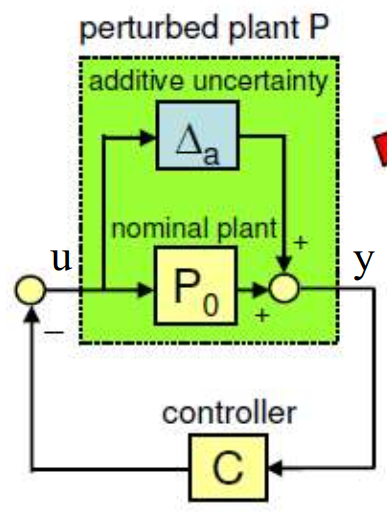
\includegraphics[width=0.5\columnwidth]{FiguresTypora/image-20220602100435357.png}
\end{center}
$$
||\Delta_a||_{\infty} < \frac{1}{||\frac{C}{1+P_0C}||_{\infty}}
$$
Plus le pic de la boucle ouverte sera faible plus on aura de possibilité de travailler avec des incertitudes.

\subsection{Perturbation multiplicative}

\begin{center}
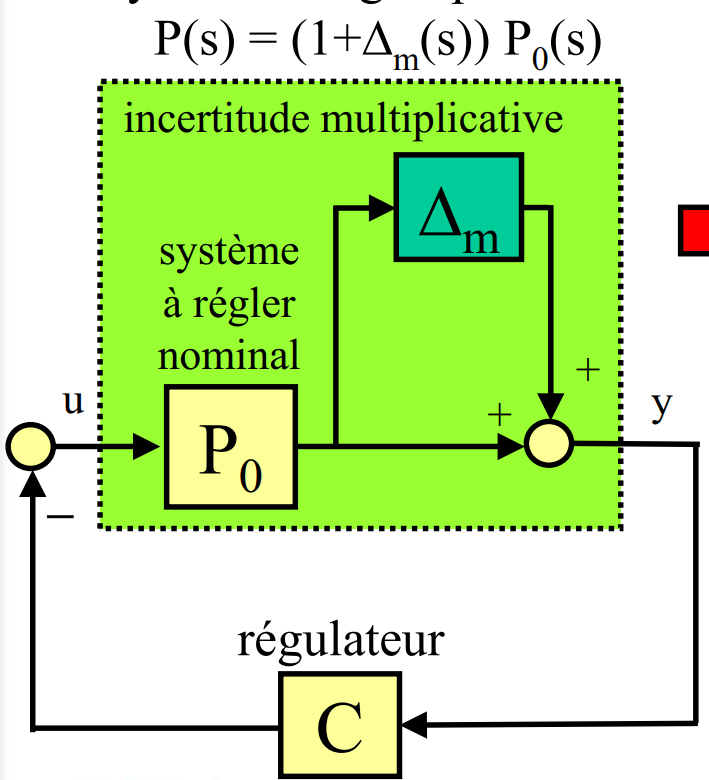
\includegraphics[width=0.5\columnwidth]{FiguresTypora/image-20220602100455177.png}
\end{center}

$$||\Delta_m||_{\infty} < \frac{1}{||\frac{P_0C}{1+P_0C}||_{\infty}}= \frac{1}{||T||_{\infty}}$$
Bruit sur un capteur

\subsection{Optimisation général}

Trouver un régulateur $C(s)$ qui tolère un maximum d'incertitude $||\Delta||_{\infty}$ donc qui minimise le pic en boucle ouverte 

\end{document}